\begin{figure}[t]
  \centering
  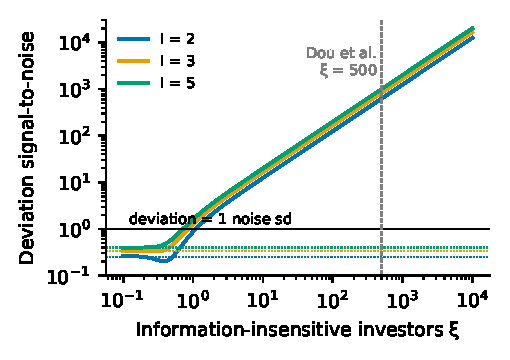
\includegraphics[width=0.55\linewidth]{figures/fig_snr.pdf}
  \caption{Signal-to-noise ratio of a one-period best-response deviation from
  the collusive intensity (order-flow change per unit of $v/\sigma_v$, in noise
  standard deviations), as a function of the mass of information-insensitive
  investors ($\sigma_v=1$, $\sigma_u=0.1$, $\theta=0.1$). Dotted lines: the
  $\xi=0$ values $(I-1)/(2I)$. Deviations become visible above noise only once
  $\xi$ exceeds about one; at the \citet{dou2025} calibration they are several
  hundred noise standard deviations large.}
  \label{fig:snr}
\end{figure}
